\chapter{Další rovinné křivky}
Nyní si můžeme definovat nejrůznější křivky sami. \\
Např. $k(t)=[t, \cos{t}], t \in \langle0, 2\pi\rangle$ je část (1 perioda) grafu funkce $\cos$,  \\
$k(t)=[\cos{t}, \cos{t}], t \in \langle0, 2\pi\rangle$ je úsečka, která leží na přímce $y=x$, \\
$k(t)=\left[\frac{1}{t}, 1-t\right], t \in (-\infty, 0) \cup (0, +\infty)$ je rovnoosá hyperbola se středem $S=[0,1]$. \\[10pt]
	Mnoho křivek je známo, některé mají i své názvy a nebo se po někom jmenují. Než si některé z nich ukážeme, zavedeme si pojmy
	\textit{singulární bod křivky} a \textit{uzlový bod křivky}. \\[10pt]
	\textbf{Singulární bod křivky} je takový bod $K=k(t_0)$, ve kterém neexistuje tečna. To nastane tehdy, když neexistuje některá
	z derivací $x'(t_0)$, $y'(t_0)$ ($k'(t)=(x'(t), y'(t))$ je tečný vektor) nebo tečný vektor je nulový, tj. $k'(t_0)=(0,0)$. \\
	Už jsme poznamenali, že délka tečného vektoru vypovídá o rychlosti, s jakou je křivka v daném bodě probíhána. Pokud je $k'(t_0)=(0,0)$,
	dojde při probíhání křivky v bodě $K=k(t_0)$ k zastavení. \\[5pt]
	\textbf{Uzlový bod křivky} je bod, kterým křivka projde vícekrát a tečny v tomto bodě jsou různé.
	\begin{figure}[H]
		\centering
		\begin{subfigure}[b]{0.4\textwidth}
			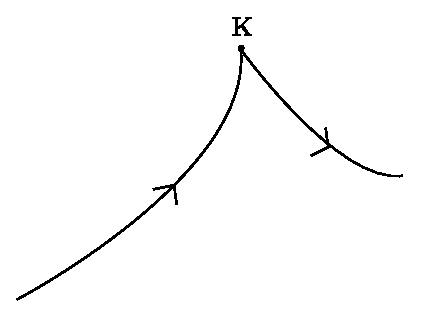
\includegraphics[width=\textwidth]{rovinnekrivky-teorie1.eps}
			\caption{Singulární bod}
		\end{subfigure}%
		\quad
		\begin{subfigure}[b]{0.4\textwidth}
			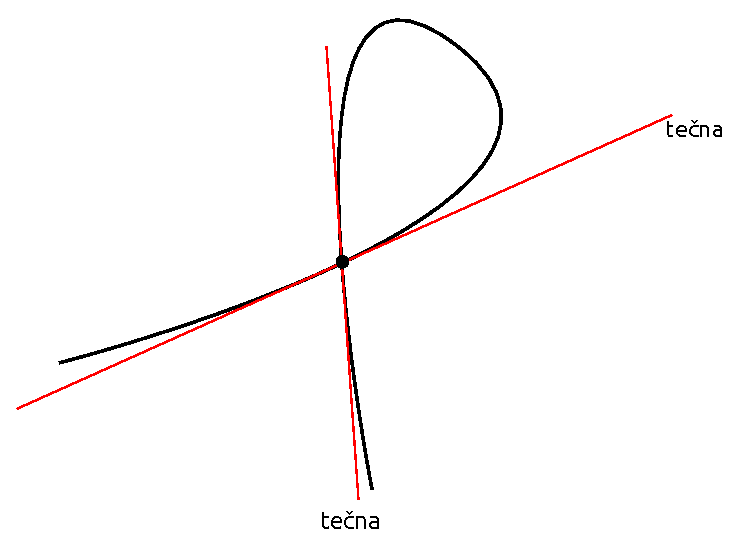
\includegraphics[width=\textwidth]{rovinnekrivky-teorie2.eps}
			\caption{Uzlový bod}
		\end{subfigure}%
	\end{figure}
	\clearpage
	\subsection*{Příklad 1}
	Je dána křivka 
	$$k(t) = \left[\cos{t} - \frac{\sqrt{2}}{2}\sin^2{t}, \cos{t}\sin{t}\right], t \in \langle0, 2\pi\rangle.$$
	Napište souřadnice singulárních bodů křivky. Dále napište parametrické i obecné rovnice tečen křivky
	v jejích průsečících s osou \textit{x}. \\[10pt]
	\textbf{Řešení:} Vypočítáme tečné vektory křivky \textit{k}, tj.:
	$$k'(t) = (-\sin{t}-\sqrt{2}\sin{t}\cos{t}, \cos^2{t}-\sin^2{t}).$$
	Abychom našli singulární body, řešíme soustavu
	$$-\sin{t}-\sqrt{2}\sin{t}\cos{t}=0$$
	a zároveň
	$$\cos^2{t}-\sin^2{t}=0.$$
	Můžeme najít všechna řešení rovnic na intervalu $\langle0,2\pi\rangle$ a pak udělat průnik.
	Nebo můžeme najít všechna řešení jedné rovnice na intervalu $\langle0,2\pi\rangle$ a vybrat
	z nich ta řešení, která splňují i druhou rovnici (ověříme dosazením).\\
	Jednodušší je použít druhý způsob. \\
	Vybereme rovnici
	\begin{align*}
		-\sin{t}-\sqrt{2}\sin{t}\cos{t} & = 0  \\
		-\sin{t}(1+\sqrt{2}\cos{t})     & = 0, 
	\end{align*}
	buď $\sin{t} = 0$ nebo $\cos{t}=-\frac{\sqrt{2}}{2}$.
	Všechna řešení na intervalu $\langle0,2\pi\rangle$ jsou
	$$t \in \left\{ 0, \frac{3\pi}{4}, \pi, \frac{5\pi}{4}, 2\pi \right\}.$$
	Dosazujeme postupně do rovnice $\cos^2{t}-\sin^2{t}=0$. Této rovnici vyhovují pouze
	$t_1 = \frac{3\pi}{4}$ a $t_2 = \frac{5\pi}{4}$. Singulární body jsou body
	\begin{align*}
		S_1 & = k\left(\frac{3\pi}{4}\right) = \left[-\frac{3\sqrt{2}}{4},-\frac{1}{2}\right]. \\
		S_2 & = k\left(\frac{5\pi}{4}\right) = \left[-\frac{3\sqrt{2}}{4},\frac{1}{2}\right].  
	\end{align*}
	Průsečíky s osou \textit{x} ($y=0$) vypočítáme z parametrického vyjádření křivky \textit{k}.
	$$\cos{t}\cdot\sin{t} = 0$$
	$$t\in\left\{0, \frac{\pi}{2}, \pi, \frac{3\pi}{2}, 2\pi\right\}$$
	Průsečíky křivky \textit{k} s osou \textit{x} jsou 3 body
	\begin{align*}
		P_1 & = k(\pi) = [-1,0],                                                                                 \\
		P_2 & = k\left(\frac{\pi}{2}\right) = k\left(\frac{3\pi}{2}\right) = \left[-\frac{\sqrt{2}}{2},0\right], \\
		P_3 & = k(0) = [1,0] = k(2\pi).                                                                          
	\end{align*}
	Vypočítáme tečné vektory a napíšeme rovnici tečen:
	\small
	\begin{flalign*}
		&k(\pi) = [-1.0], &\\
		&k'(\pi) = (0,1), &\\
		&p_1(s) = [-1, s],s \in \mathbb{R}\text{ parametrická rovnice}, &\\
		&p_1: x=-1\text{ obecná rovnice}, &\\
		&k\left(\frac{3\pi}{2}\right) = \left[-\frac{\sqrt{2}}{2},0\right], &\\
		&k'\left(\frac{3\pi}{2}\right) = (1,-1), &\\
		&p_2(s) = \left[-\frac{\sqrt{2}}{2}+s,-s\right],s \in \mathbb{R}, &\\
		&p_2: x+y+\frac{\sqrt{2}}{2}=0, &\\
		&k\left(\frac{\pi}{2}\right) = \left[-\frac{\sqrt{2}}{2},0\right], &\\
		&k'\left(\frac{\pi}{2}\right) = (-1,-1) \sim (1,1), &\\
		&q_2(s) = \left[-\frac{\sqrt{2}}{2}+s,s\right],s \in \mathbb{R}, &\\
		&q_2: x-y+\frac{\sqrt{2}}{2}=0,\\
	\end{flalign*}
	bod $\left[-\frac{\sqrt{2}}{2}, 0\right]$ je uzlový bod křivky \textit{k}, \\
	\begin{flalign*}
		&k(0) = [1,0] = k(2\pi), &\\
		&k'(0) = k'(2\pi) = (0,1), &\\
		&p_3(s) = [1, s],s \in \mathbb{R}, &\\
		&p_3: x=1. &\\
	\end{flalign*}	 
	\normalsize
	Nakreslíme-li zadanou křivku, vidíme na obrázku singulární body (špičky) i uzlový bod. Je také jasné
	proč se křivka nazývá \uv{ryba} (\textit{fish curve}).
	\begin{figure}[H]
		\centering
		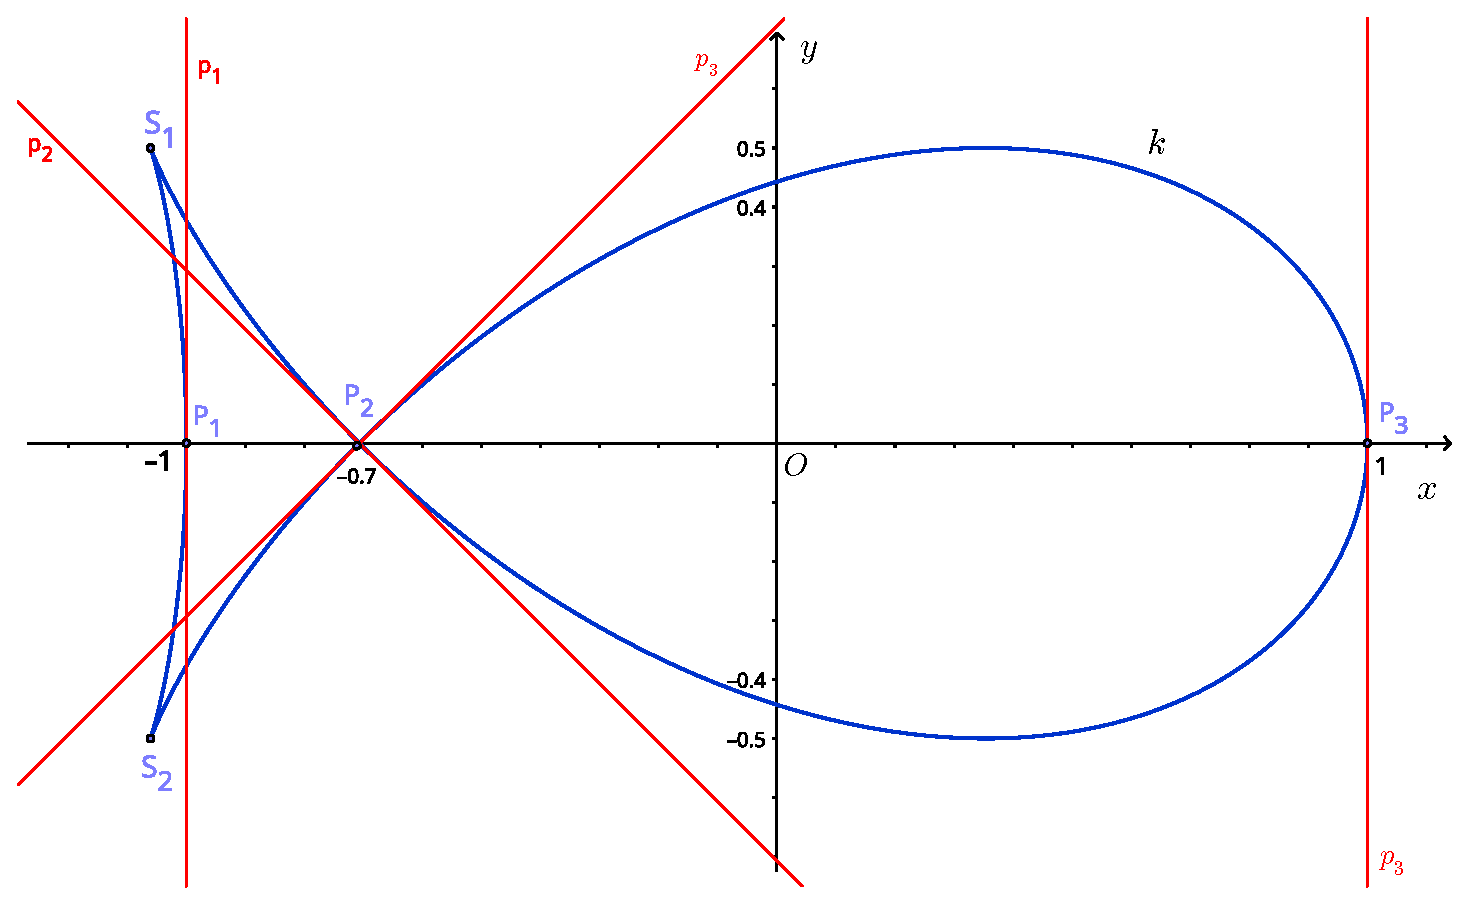
\includegraphics[width=\textwidth]{rovinnakrivka1-geo.eps}
		\caption{Fish curve pro $t \in \langle0, 2\pi\rangle$}
		
	\end{figure}
	\clearpage 		 
	\subsection*{Příklad 2}
	Je dána křivka
	$$k(t) = [16\sin^3{t}, 13\cos{t}-5\cos{2t}-2\cos{3t}-\cos{4t}], t \in \langle0, 2\pi\rangle.$$
	Napište souřadnice singulárních bodů křivky. Dále napište souřadnice bodů křivky, ve kterých
	má křivka tečny rovnoběžné s osou \textit{y}, napište obecné rovnice těchto tečen. \\[10pt]
	\textbf{Řešení:} Vypočítáme tečné vektory křivky \textit{k}, tj.:
	$$k'(t) = (48\sin^2{t}\cos{t},-13\sin{t}+10\sin{2t}+6\sin{3t}+4\sin{4t}).$$
	Abychom našli singulární body, řešíme soustavu rovnic
	$$48\sin^2{t}\cos{t}=0$$
	a zároveň
	$$-13\sin{t}+10\sin{2t}+6\sin{3t}+4\sin{4t}=0.$$
	Najdeme všechna řešení první rovnice na intervalu $\langle0, 2\pi\rangle$, jsou to
	$t \in \left\{ 0, \frac{\pi}{2}, \pi, \frac{3\pi}{2}, 2\pi \right\}$. \\
	Tato řešení dosazujeme do druhé rovnice, druhé rovnici vyhovují 3 hodnoty
	$t_1=0$, $t_2=\pi$ a $t_3=2\pi$. \\
	Křivka má dva singulární body:
	\begin{align*}
		S_1 & = k(0) = k(2\pi)=[0, 5], \\
		S_2 & = k(\pi) = [0, -17].     
	\end{align*}
	Tečný vektor je rovnoběžný s osou \textit{y}, je-li jeho první složka nulová a druhá nenulová.
	To nastane pro hodnoty $t_4=\frac{\pi}{2}$ a $t_5=\frac{3\pi}{2}$.
	Obecné rovnice tečen rovnoběžných s osou \textit{y} jsou:
	\begin{align*}
		k\left(\frac{3\pi}{2}\right)  & = [-16,4] = P_1, \\
		k'\left(\frac{3\pi}{2}\right) & = (0, 19),       \\
		p_1: x                        & = -16            
	\end{align*}
	a
	\begin{align*}
		k\left(\frac{\pi}{2}\right)  & = [16,4] = P_2, \\
		k'\left(\frac{\pi}{2}\right) & = (0, -19),     \\
		p_2: x                       & = 16.           
	\end{align*}
	\clearpage
	\noindent Nakreslíme-li zadanou křivku, vidíme na obrázku singulární body (špičky na křivce). Tato křivka se nazývá \uv{srdce} (\textit{heartcurve}) a řadíme ji mezi další křivky, které se často souhrnně označují \textit{srdcovky}.
	\begin{figure}[H]
		\centering
		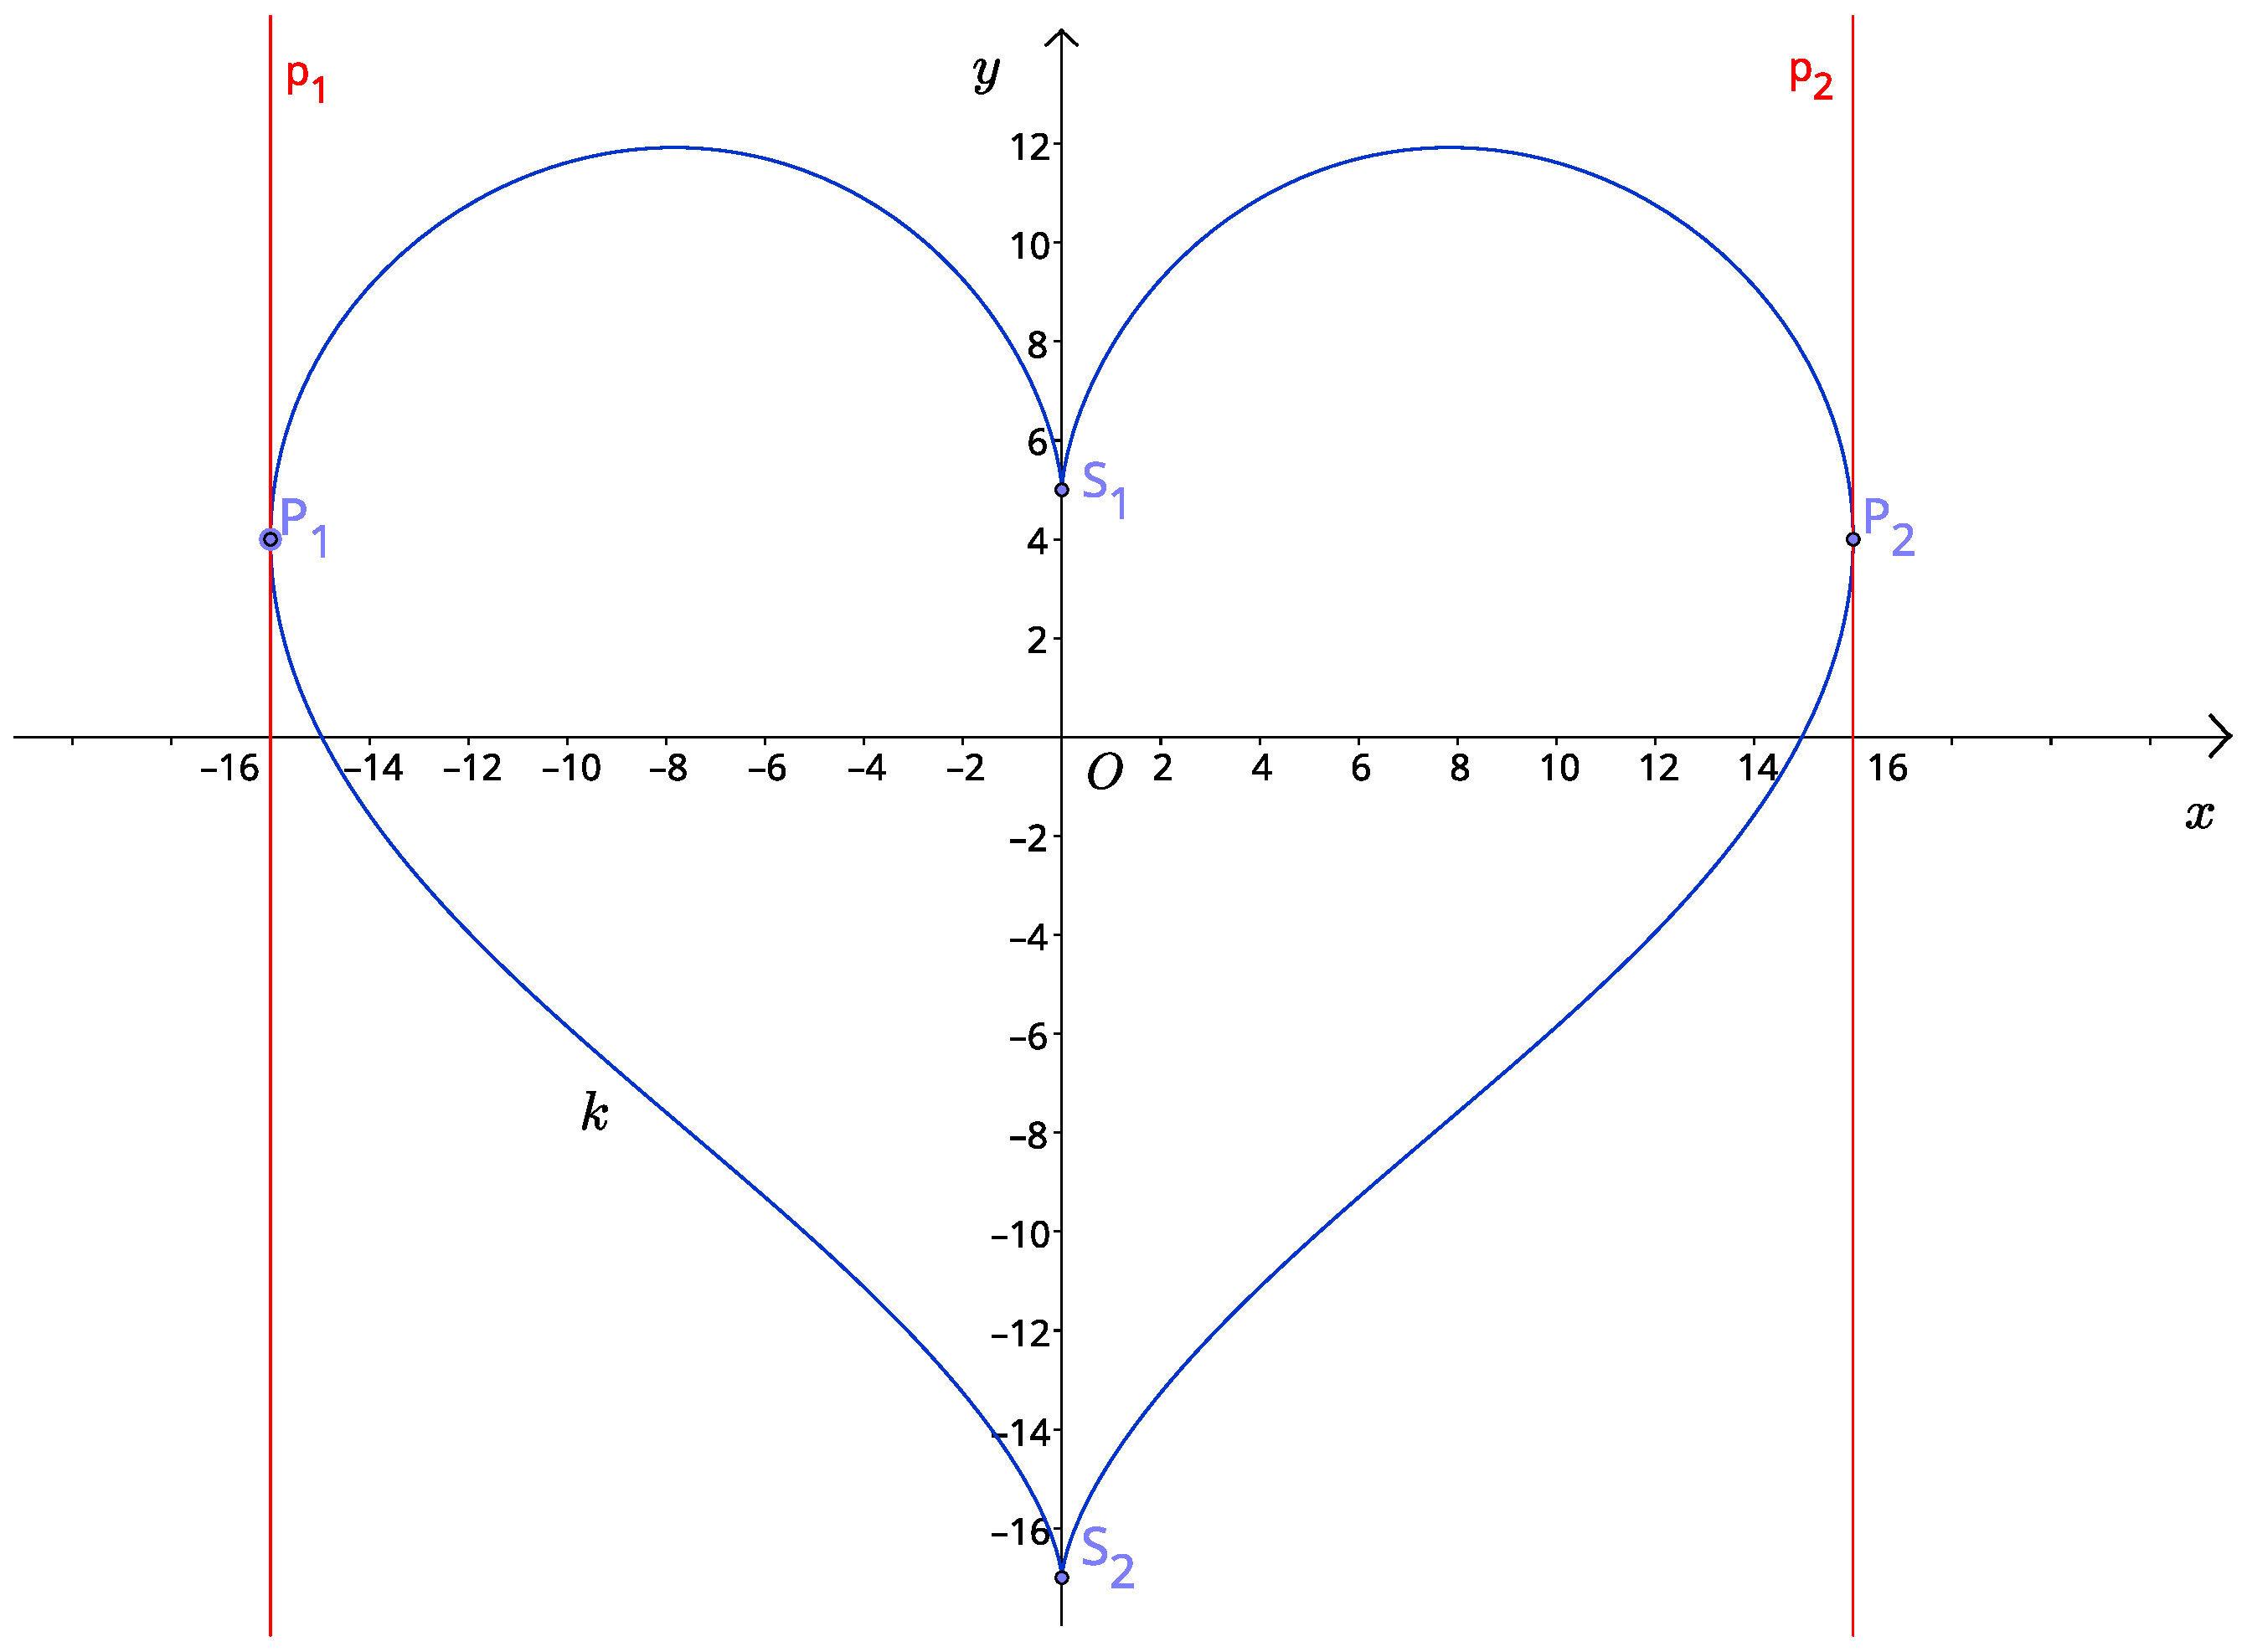
\includegraphics[width=\textwidth]{rovinnakrivka2-geo.eps}
		\caption{Rovinná křivka pro $t \in \langle0, 2\pi\rangle$}
		
	\end{figure}	